% ===========================================================================
% Figure blocks for the JMLR-format paper.
%
% PREAMBLE: add this line after \usepackage{jmlr2e}. graphicx is already
% loaded by jmlr2e, so it does not need to be added again. The two paths mean
% the same source works whether the PNGs sit in ./figures/ (e.g. Overleaf) or
% you are building inside the repository next to report/figures/.
%
%   \graphicspath{{figures/}{../report/figures/}}
%
% No other package is required: the two-panel figures below use plain
% minipages, not subcaption.
% ===========================================================================


% --- Figure 1: the main result -- the sign reversal -------------------------
% Panels stacked, because these plots are wide (1500x810) and shrinking them
% to half a column makes the axis labels unreadable. This figure is tall; if
% it crowds the page, drop both widths to 0.88\textwidth.

\begin{figure}[p]
\centering
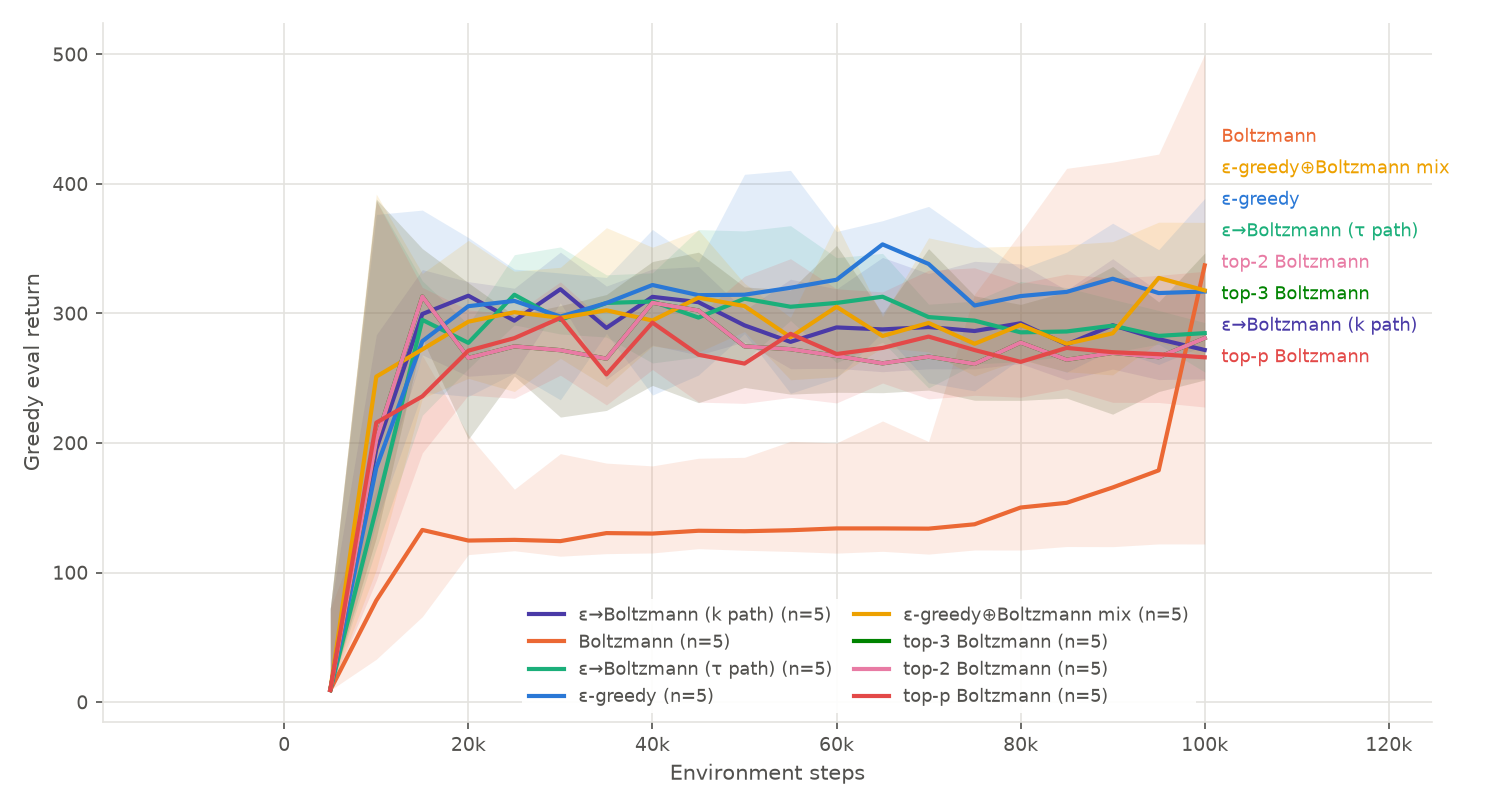
\includegraphics[width=\textwidth]{full_gym_CartPole-v1_curves.png}\\[1.5ex]
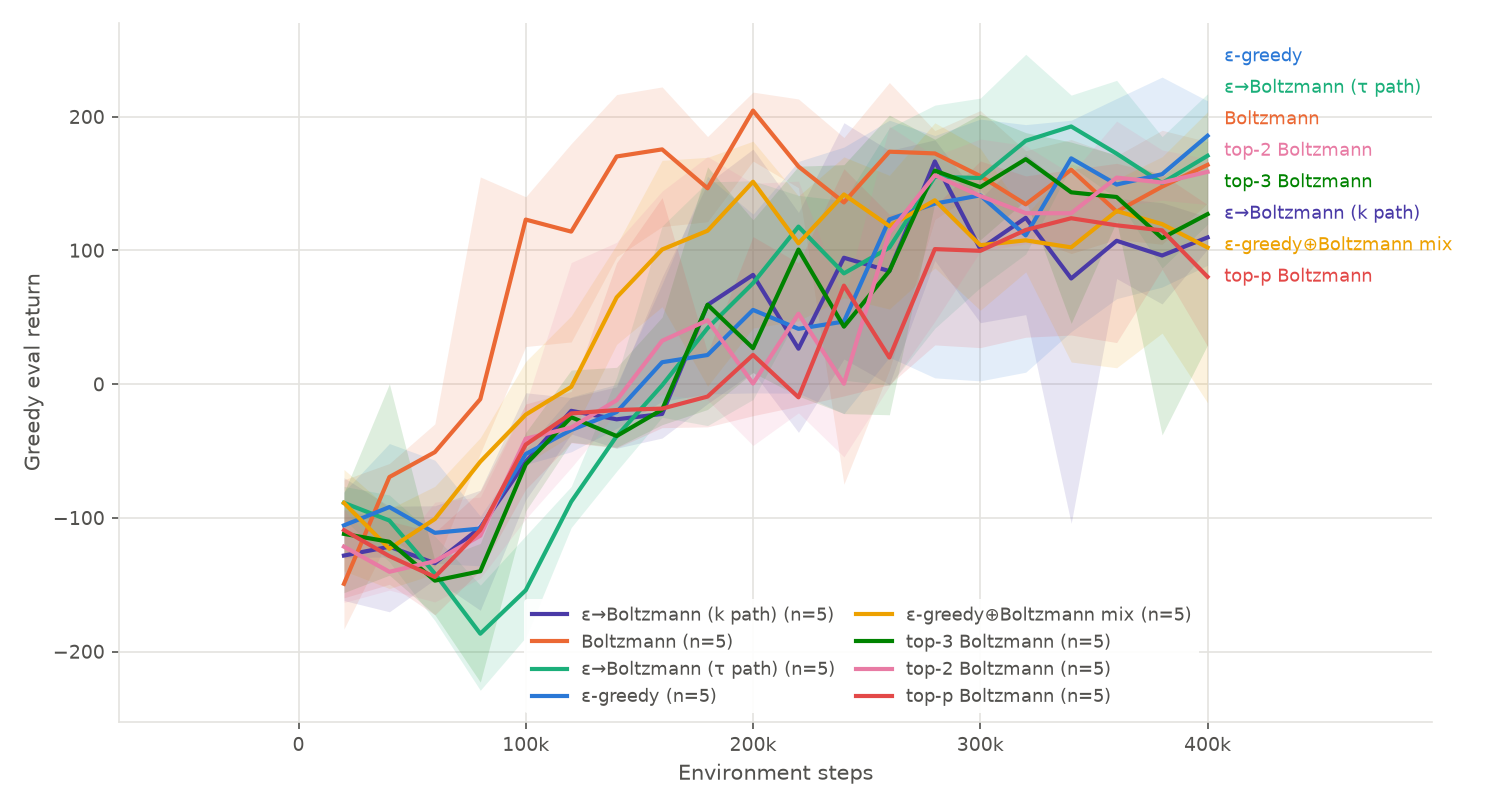
\includegraphics[width=\textwidth]{full_gym_LunarLander-v3_curves.png}
\caption{Learning curves, IQM over five seeds with 95\% stratified bootstrap
bands. \textbf{Top:} CartPole-v1, 100k steps, $|A| = 2$. \textbf{Bottom:}
LunarLander-v3, 400k steps, $|A| = 4$. Boltzmann without an $\varepsilon$
floor (orange) is the slowest learner on CartPole and the fastest on
LunarLander, overtaking every other variant between 80k and 250k steps. The
same rule, the same code, opposite behaviour: the value of the uniform
$\varepsilon$ floor reverses sign between these two environments.}
\label{fig:curves}
\end{figure}


% --- Figure 2: the one resolved comparison among the annealing variants -----

\begin{figure}[t]
\centering
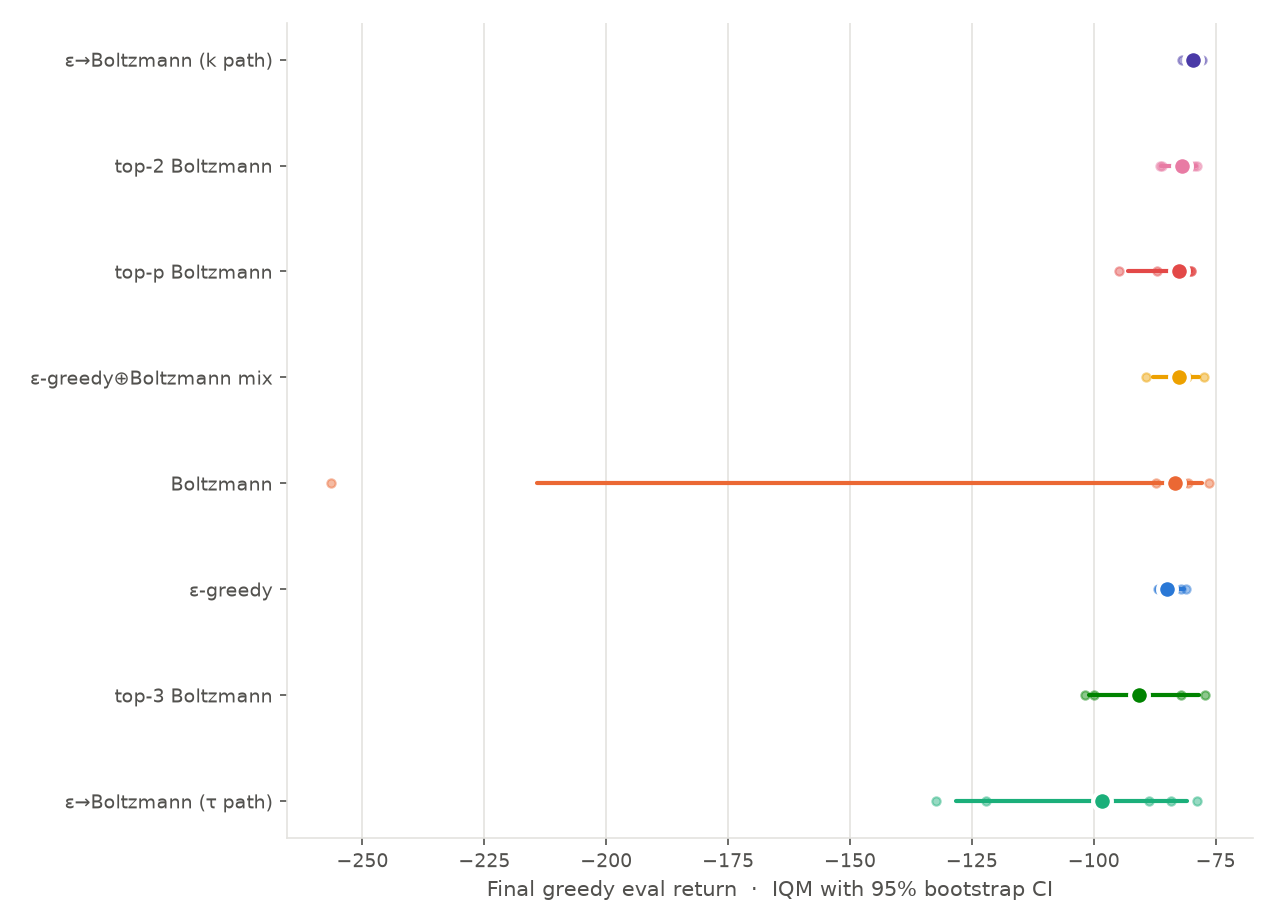
\includegraphics[width=0.85\textwidth]{full_gym_Acrobot-v1_final.png}
\caption{Final performance on Acrobot-v1 (150k steps, $|A| = 3$), IQM with
95\% stratified bootstrap confidence intervals over five seeds; the small
faint dots are the individual seeds. The support path (\texttt{anneal\_k},
where $k$ grows from $1$ to $|A|$ at fixed temperature) is the only variant
that separates from the $\varepsilon$-greedy baseline, with a probability of
improvement of $0.96$ $[0.76, 1.00]$. Note that the temperature path is at the
same time the worst variant here, so the effect belongs to the support path
specifically rather than to annealing in general.}
\label{fig:acrobot-final}
\end{figure}


% --- Figure 3: the mechanism behind Figure 1 -------------------------------

\begin{figure}[t]
\centering
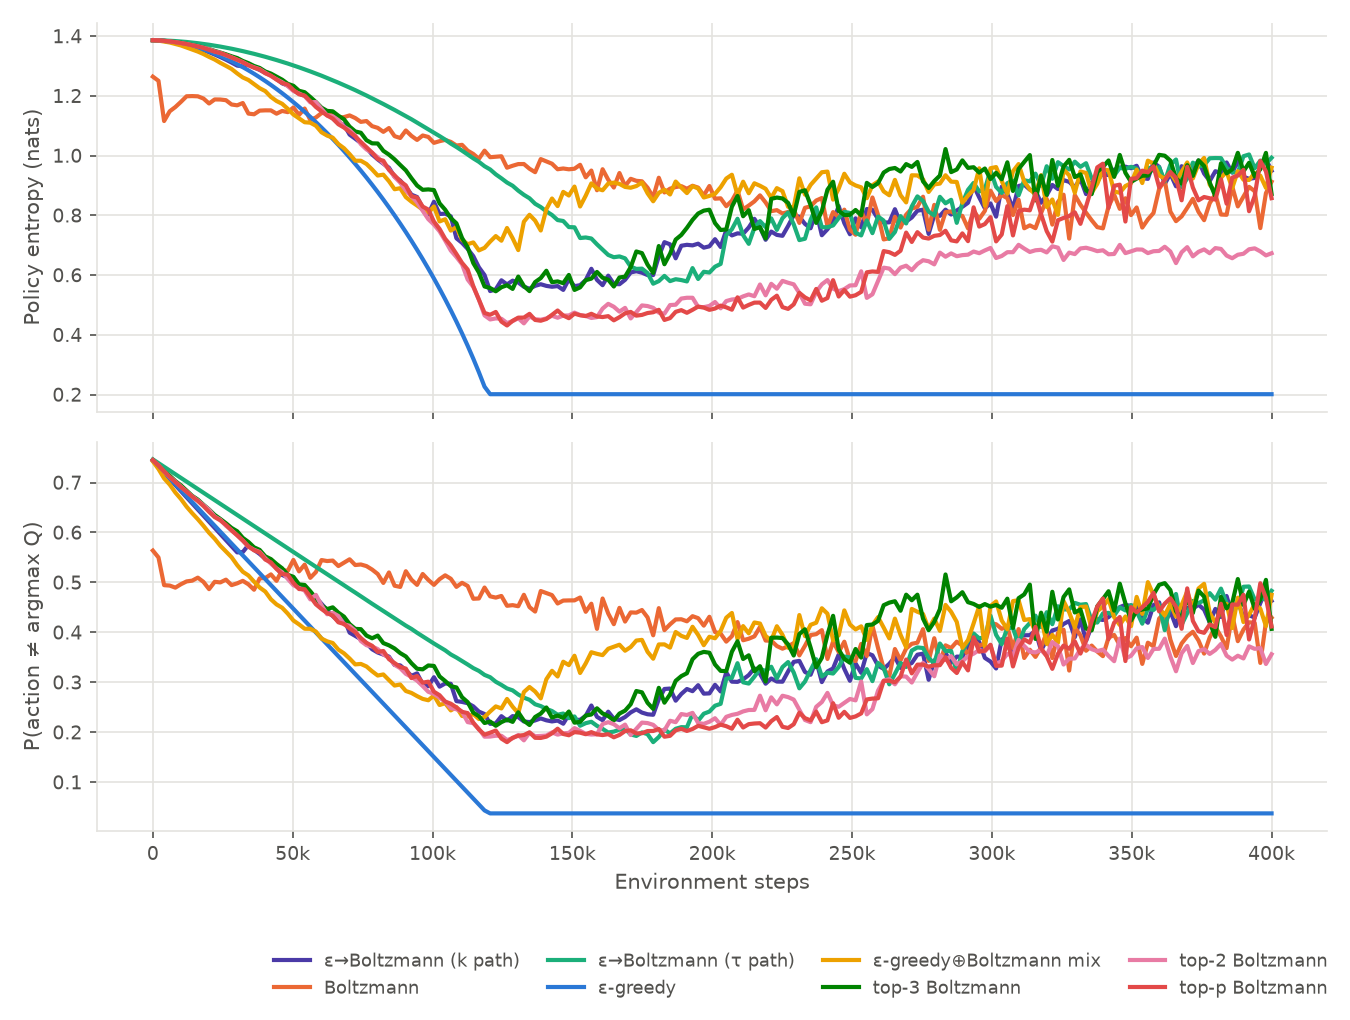
\includegraphics[width=0.9\textwidth]{full_gym_LunarLander-v3_exploration.png}
\caption{Behaviour-policy exploration on LunarLander-v3, mean over five seeds.
\textbf{Top:} policy entropy, where the maximum for four actions is
$\ln 4 = 1.39$ nats. \textbf{Bottom:} probability of taking a non-greedy
action. Once its schedule ends at 120k steps, $\varepsilon$-greedy (blue)
collapses to $0.20$ nats and stays there, while every Boltzmann variant keeps
roughly $0.9$ nats of exploration for the remaining 280k steps. On LunarLander
a uniformly random action fires thrusters at random and crashes the lander, so
$\varepsilon$-greedy is spending its exploration budget on actions already
known to be catastrophic. This is the mechanism behind
Figure~\ref{fig:curves}.}
\label{fig:exploration}
\end{figure}


% --- Figure 4: Q-scale ablation --------------------------------------------

\begin{figure}[t]
\centering
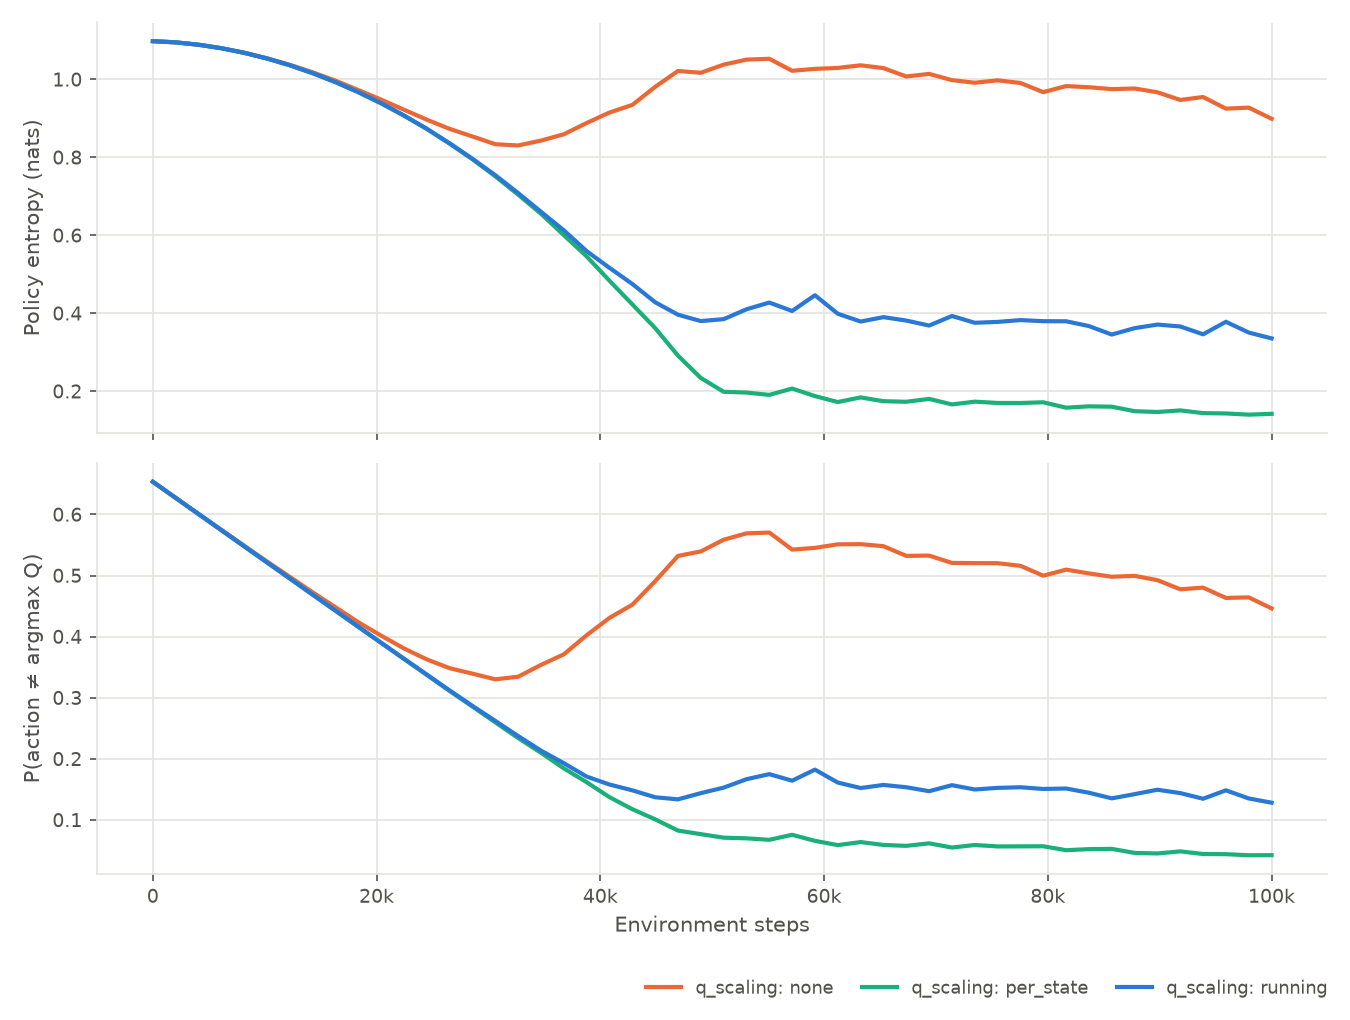
\includegraphics[width=0.9\textwidth]{ablation_scaling_Acrobot-v1_exploration.png}
\caption{Q-value scale normalisation ablation on Acrobot-v1, temperature-path
schedule, mean over three seeds. Without normalisation (\texttt{none}, orange)
the entropy turns back \emph{upward} at 30k steps and never settles: as the
Q-values inflate during training, a fixed $\tau$ keeps meaning something
different, so the one number that is supposed to control Boltzmann exploration
is not actually under the experimenter's control. \texttt{running} settles at
$0.34$ nats and \texttt{per\_state} at $0.14$, the latter being roughly
$2.5\times$ more confidently peaked because forcing every Q-row to unit spread
manufactures a preference even where the actions are equivalent. This
separation reproduced to within $0.04$ nats on a second machine, while the
performance ranking of the very same runs did not reproduce at all.}
\label{fig:ablation}
\end{figure}


% --- Figure 5: the uncertainty-gated extension -----------------------------

\begin{figure}[t]
\centering
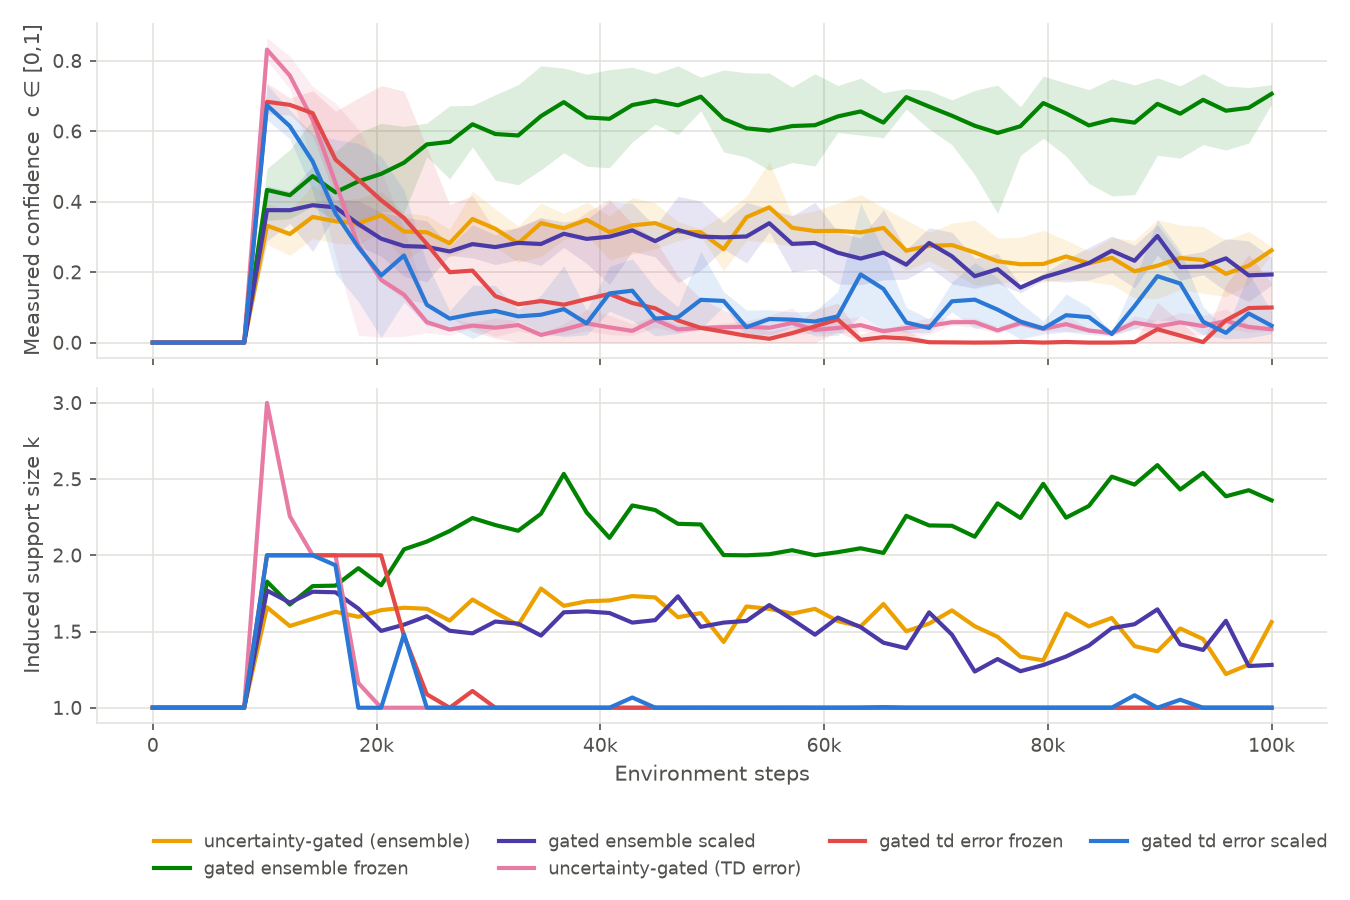
\includegraphics[width=0.9\textwidth]{uncertainty_Acrobot-v1_confidence.png}
\caption{Uncertainty-gated handover on Acrobot-v1, mean over three seeds with
bootstrap bands. \textbf{Top:} the measured confidence $c \in [0,1]$ that
drives the knobs. \textbf{Bottom:} the support size $k$ that confidence
induces. Confidence is held at $0$ during a 10k-step warm-up. After it, only
the frozen-reference variant (green) produces a confidence that rises and a
support that widens from $1$ to about $2.4$: the handover the extension exists
to perform. Every variant that normalises the signal against a running
quantile of the signal's own history is pinned below $c = 0.35$ for the whole
run, because the reference tracks the signal and cancels exactly the trend the
gate is meant to detect.}
\label{fig:uncertainty}
\end{figure}


% ===========================================================================
% ALTERNATIVE for Figure 1: panels side by side.
% Only worth it if you shrink the source figures first -- at half a column the
% current legends are about 3pt tall. Requires \usepackage{subcaption}.
% ===========================================================================
%
% \begin{figure}[t]
% \centering
% \begin{subfigure}[b]{0.49\textwidth}
%   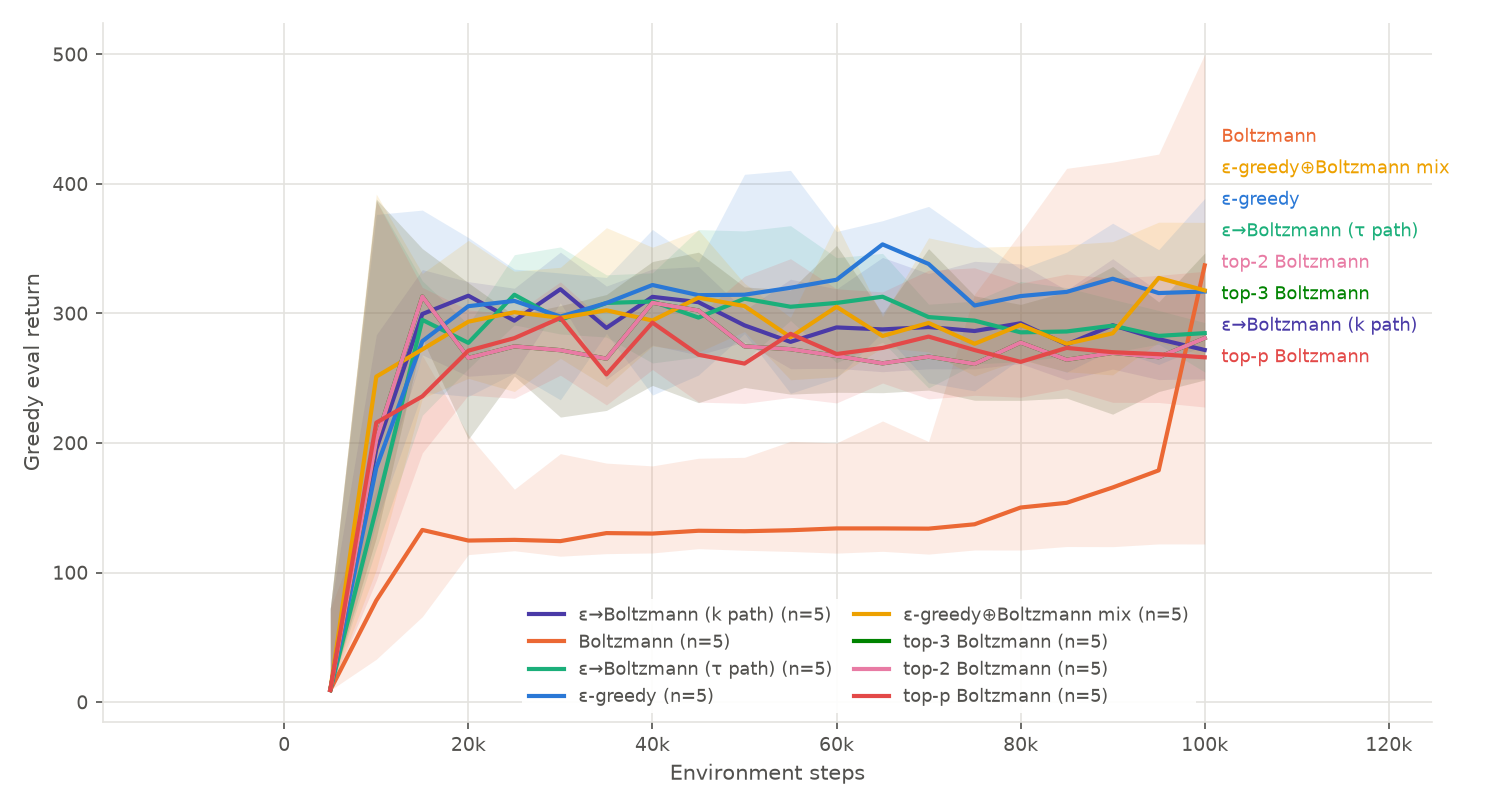
\includegraphics[width=\textwidth]{full_gym_CartPole-v1_curves.png}
%   \caption{CartPole-v1 ($|A| = 2$)}
%   \label{fig:curves-cartpole}
% \end{subfigure}
% \hfill
% \begin{subfigure}[b]{0.49\textwidth}
%   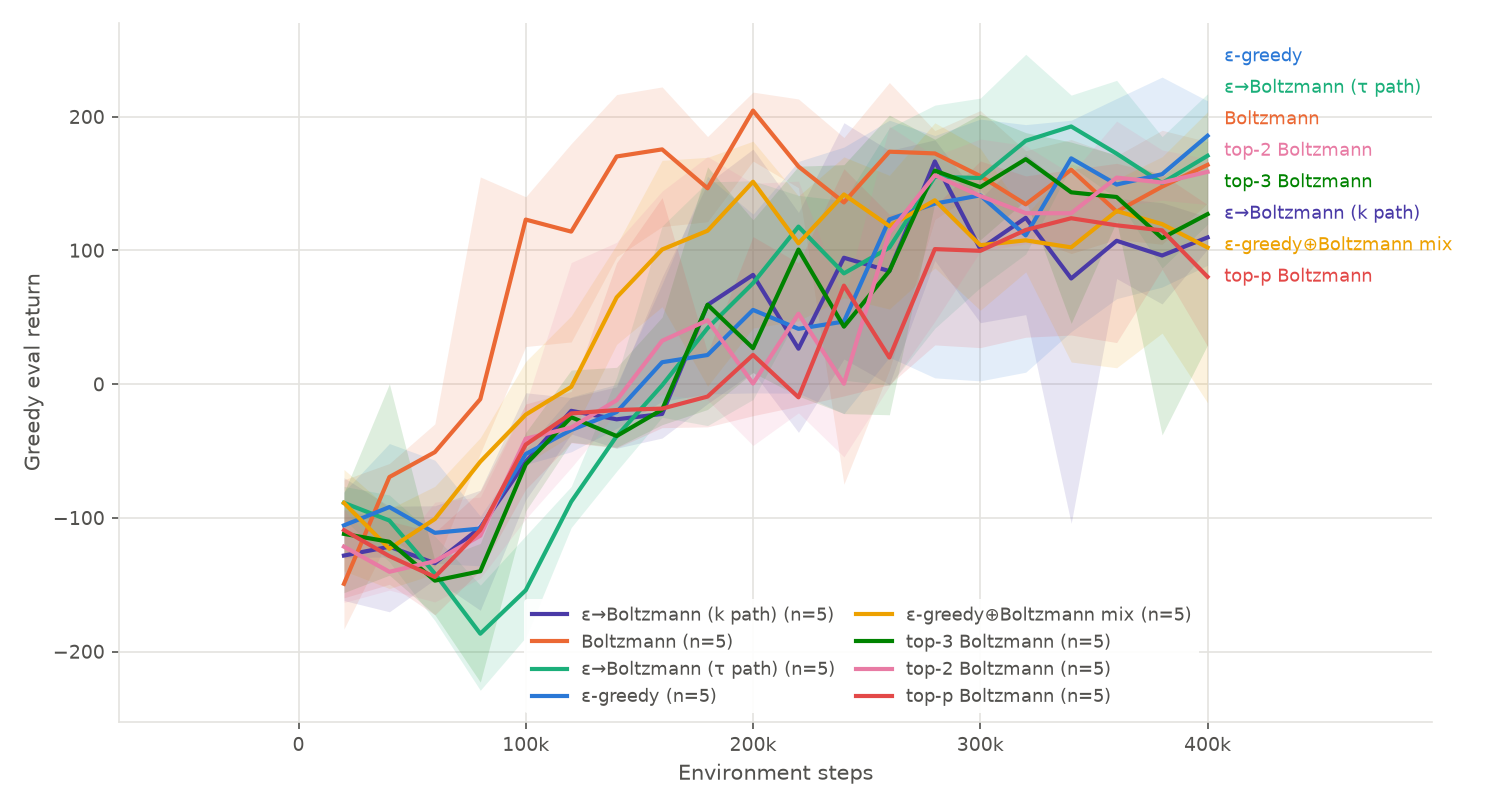
\includegraphics[width=\textwidth]{full_gym_LunarLander-v3_curves.png}
%   \caption{LunarLander-v3 ($|A| = 4$)}
%   \label{fig:curves-lunarlander}
% \end{subfigure}
% \caption{...}
% \label{fig:curves}
% \end{figure}
